\chapter{Introduction}
\setlength{\parskip}{2.5ex plus .4ex minus .4ex}
\section{Context}
\subsection{National Institute of Informatics}
The NII\footnote{National Institute of Informatics} of Tokyo is an inter university research institute which aim to develop the research in multiple domains. The Institute is focused on fields including networking software and content.
The NII is composed by several laboratories which work on different international research project. One of them is directed by the associate professor Inamura Tetsunari where I am doing my internship.\\
The Inamura laboratory works on several project, which one is SIGVerse, a simulator.

\subsection{SIGVerse}
SIGVerse is a virtual world which can model objects and agents.\\
This simulator has been created to give a tool for studying interactions between agents but also comprehension and knowledge in many fields.\\
Understanding the mechanism of intelligence of human being is the key to develop intelligent robot system. That's why this simulator is very useful.\\
The movement of the user can be reproduced in the virtual world thanks to the kinect and the representation of the world can be projected on the oculus. So, the user can be ``inside'' the simulator and interact more easily with its.\\
We can see in figure~\ref{fig:manVirtualWorld}, the representation of an agent. This agent could be a robot too, and it is possible to program its movements or send to it a message to execute an action. That's why this simulator is well adapted to host the training and virtual competition of Robocup.\\
However, the use of the simulator is exclusively for SIGVerse users which limits its growth.\\

\noindent\begin{minipage}{\linewidth}% to keep image and caption on one page
\makebox[\linewidth]{%        to center the image
  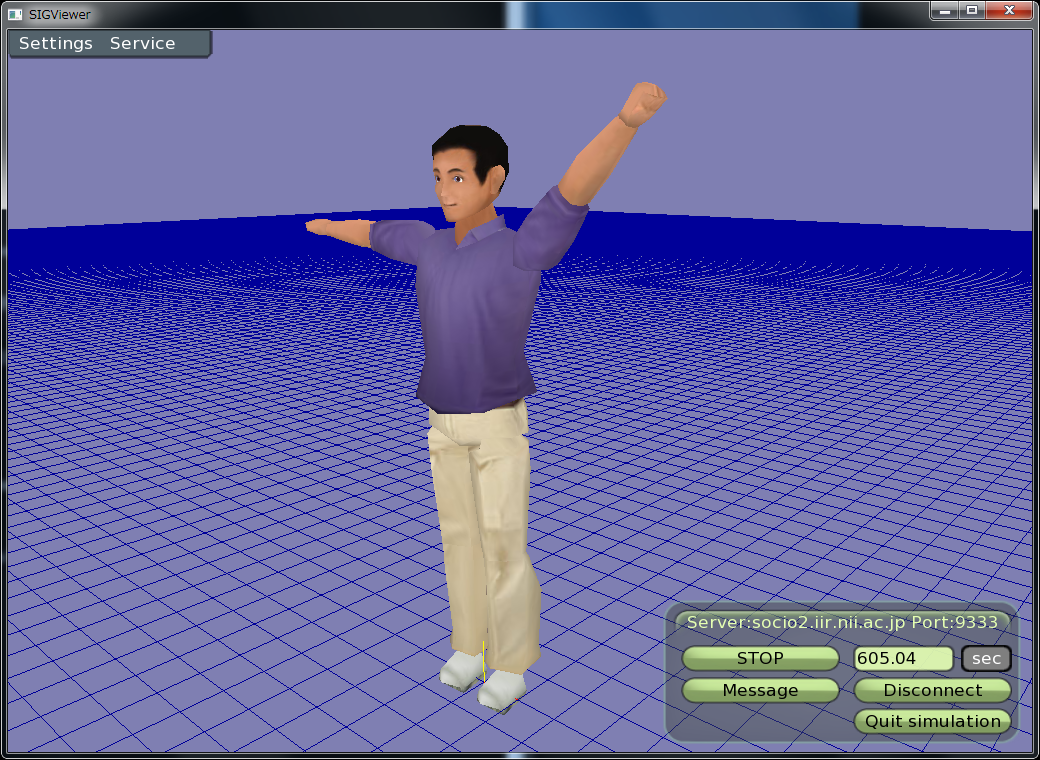
\includegraphics [width=100mm]{images/manViewer.png}}
\captionof{figure}{Simple agent in the virtual world}\label{fig:manVirtualWorld}%      only if needed  
\end{minipage}

\section{Topic}
SIGVerse is limited to SIGVerse users. This topic has the goal to growth the SIGVerse community by joining the ROS\footnote{Robot Operating System} community.\\
This gathering has been chosen because of several reasons.\\
First of all ROS is open source like SIGVerse and has a big community who works on robots. Then ROS can provide a collection of tools, libraries, and conventions that aim to simplify the task of creating complex and robust robot behavior across a wide variety of robotic platforms.\\
ROS make possible to manage a robot as SIGVerse do but there is advantages to using ROS. Indeed, ROS is designed to be as distributed and modular as possible so, it encourages the collaboration to develop robot software whereas SIGVerse is not.\\

In this report, I am going to detail the suggested work, general idea and how ROS works. After that, I am going to detail what I started doing, architecture, topics, services, troubles...